
%%%%%%%%%%%%%%%%%%%%%%%%%%%%%%%%%%%%%%%%%%%%%%%%%%%%%%%%%%%%%%%%%%%%%%%%%%%%%%%
\subsection{Phenoregions}
%%%%%%%%%%%%%%%%%%%%%%%%%%%%%%%%%%%%%%%%%%%%%%%%%%%%%%%%%%%%%%%%%%%%%%%%%%%%%%%
\begin{frame}
 \frametitle{Clustering MODIS NDVI into Phenoregions}
 \vskip-0.10in
 \begin{itemize}\small
  \item Hoffman and Hargrove previously used $k$-means clustering to detect brine scars from hyperspectral data \citep{Hoffman_MS-UTK-Physics_20041104} and to classify phenologies from monthly climatology and 17 years of 8~km NDVI from AVHRR \citep{White_GRL_20050218}.
  \item This data mining approach requires high performance computing to analyze the entire body of the high resolution MODIS NDVI record for the continental U.S.
  \item {\color{blue} $>$87B NDVI values}, consisting of {\color{blue} $\sim$146.4M cells} for the CONUS at 250~m resolution with \textcolor{blue}{46 maps per year} for \textcolor{blue}{13~years} (2000--2012), analyzed using $k$-means clustering.
  \item The annual traces of NDVI for every year and map cell are combined into one \textcolor{blue}{327~GB single-precision binary} data set of 46-dimensional observation vectors.
  \item Clustering yields 13 phenoregion maps in which each cell is classified into one of $k$ phenoclasses that represent prototype annual NDVI traces.
 \end{itemize}
\end{frame}
%%%%%%%%%%%%%%%%%%%%%%%%%%%%%%%%%%%%%%%%%%%%%%%%%%%%%%%%%%%%%%%%%%%%%%%%%%%%%%%

%%%%%%%%%%%%%%%%%%%%%%%%%%%%%%%%%%%%%%%%%%%%%%%%%%%%%%%%%%%%%%%%%%%%%%%%%%%%%%%
\begin{frame}
 \frametitle{50 Phenoregions for year 2012 (Random Colors)}
 \includegraphics[width=\textwidth]{figures/phendump.2000-2012.50.2012.large.GIMP.pdf}
\end{frame}
%%%%%%%%%%%%%%%%%%%%%%%%%%%%%%%%%%%%%%%%%%%%%%%%%%%%%%%%%%%%%%%%%%%%%%%%%%%%%%%

%%%%%%%%%%%%%%%%%%%%%%%%%%%%%%%%%%%%%%%%%%%%%%%%%%%%%%%%%%%%%%%%%%%%%%%%%%%%%%%
\begin{frame}
 \frametitle{50 Phenoregion Prototypes (Random Colors)}
 \begin{center}
  \begin{columns}
   \begin{column}{0.01\textwidth}
    \begin{sideways}\vbox{\Large NDVI}\end{sideways}
   \end{column}
   \hspace{-0.3in}
   \begin{column}{0.95\textwidth}
    \includegraphics[width=\textwidth,trim=1in 6.5in 1in 1in,clip=true]{figures/paintchips.phendump.2000-2012.50.pdf} \\
    \vskip-0.15in
    \centerline{\Large day of year}
   \end{column}
  \end{columns}
 \end{center}
\end{frame}
%%%%%%%%%%%%%%%%%%%%%%%%%%%%%%%%%%%%%%%%%%%%%%%%%%%%%%%%%%%%%%%%%%%%%%%%%%%%%%%

%%%%%%%%%%%%%%%%%%%%%%%%%%%%%%%%%%%%%%%%%%%%%%%%%%%%%%%%%%%%%%%%%%%%%%%%%%%%%%%
\begin{frame}
 \frametitle{50 Phenoregions Persistence}
 \includegraphics[width=\textwidth]{figures/phendump.2000-2012.50.persistence.large.GIMP.pdf}
\end{frame}
%%%%%%%%%%%%%%%%%%%%%%%%%%%%%%%%%%%%%%%%%%%%%%%%%%%%%%%%%%%%%%%%%%%%%%%%%%%%%%%

%%%%%%%%%%%%%%%%%%%%%%%%%%%%%%%%%%%%%%%%%%%%%%%%%%%%%%%%%%%%%%%%%%%%%%%%%%%%%%%
\begin{frame}
 \frametitle{50 Phenoregions Mode (Random Colors)}
 \includegraphics[width=\textwidth]{figures/phendump.2000-2012.50.mode.large.GIMP.pdf}
\end{frame}
%%%%%%%%%%%%%%%%%%%%%%%%%%%%%%%%%%%%%%%%%%%%%%%%%%%%%%%%%%%%%%%%%%%%%%%%%%%%%%%

%%%%%%%%%%%%%%%%%%%%%%%%%%%%%%%%%%%%%%%%%%%%%%%%%%%%%%%%%%%%%%%%%%%%%%%%%%%%%%%
\begin{frame}
 \frametitle{50 Phenoregions Max Mode (Random Colors)}
 \includegraphics[width=\textwidth]{figures/phendump.2000-2012.50.maxmode.large.GIMP.pdf}
\end{frame}
%%%%%%%%%%%%%%%%%%%%%%%%%%%%%%%%%%%%%%%%%%%%%%%%%%%%%%%%%%%%%%%%%%%%%%%%%%%%%%%

%%%%%%%%%%%%%%%%%%%%%%%%%%%%%%%%%%%%%%%%%%%%%%%%%%%%%%%%%%%%%%%%%%%%%%%%%%%%%%%
\begin{frame}
 \frametitle{50 Phenoregions Max Mode (Similarity Colors)}
 \includegraphics[width=\textwidth]{figures/phendump.2000-2012.50.maxmode.sim.GIMP.pdf}
% phendump.2000-2011.50.maxmode.sim_gimp.pdf}
\end{frame}
%%%%%%%%%%%%%%%%%%%%%%%%%%%%%%%%%%%%%%%%%%%%%%%%%%%%%%%%%%%%%%%%%%%%%%%%%%%%%%%

%%%%%%%%%%%%%%%%%%%%%%%%%%%%%%%%%%%%%%%%%%%%%%%%%%%%%%%%%%%%%%%%%%%%%%%%%%%%%%%
\begin{frame}
 \frametitle{50 Phenoregions Max Mode (Similarity Colors Legend)}
 \begin{center}
  \vskip-0.30in
  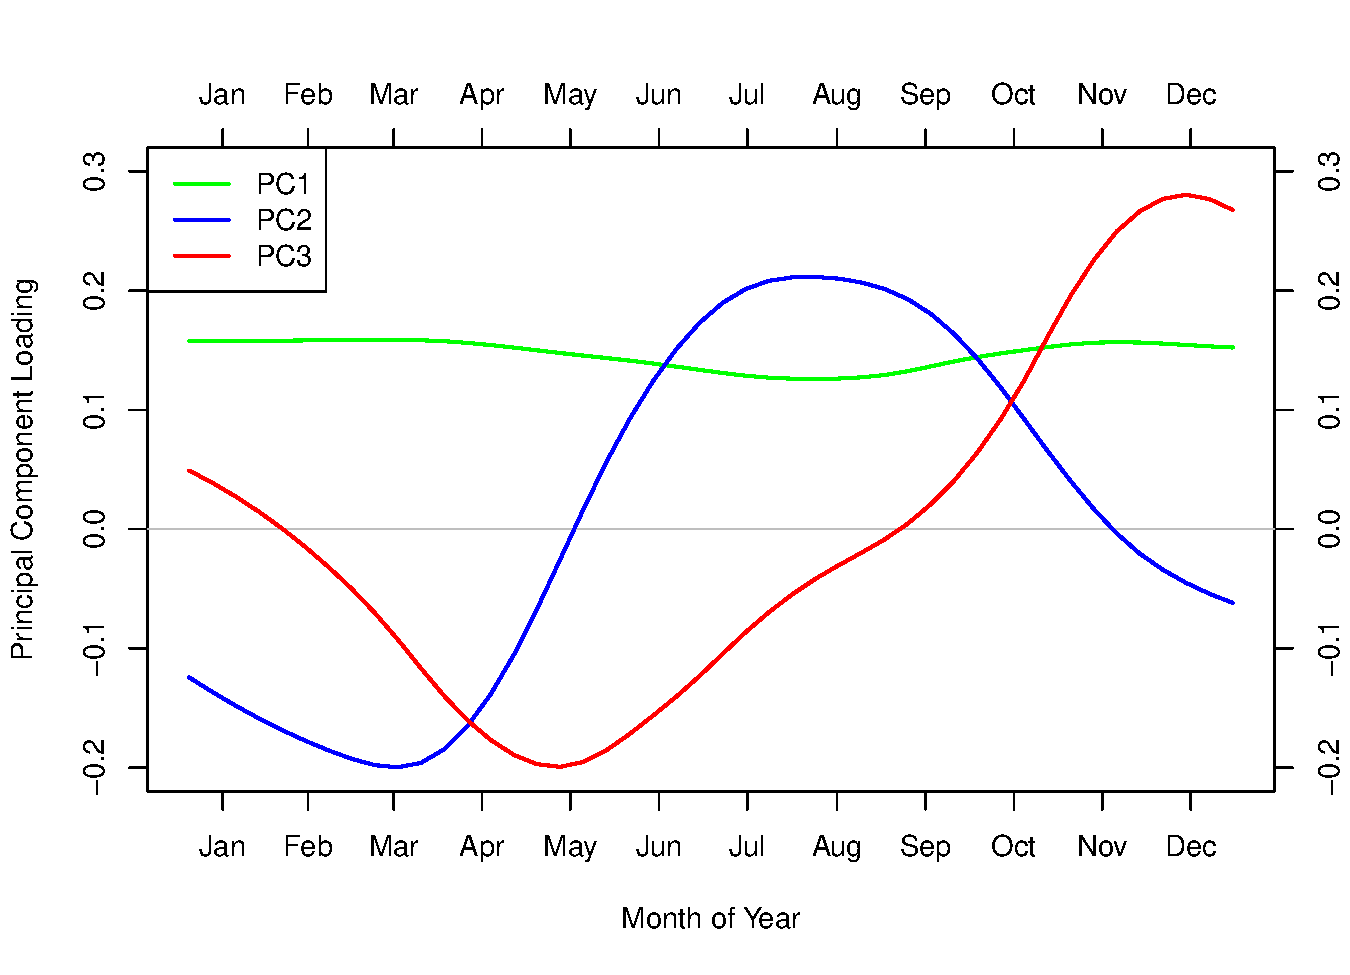
\includegraphics[width=\textwidth]{figures/phenology_2000-2012_pc.pdf}
 \end{center}
\end{frame}
%%%%%%%%%%%%%%%%%%%%%%%%%%%%%%%%%%%%%%%%%%%%%%%%%%%%%%%%%%%%%%%%%%%%%%%%%%%%%%%

%%%%%%%%%%%%%%%%%%%%%%%%%%%%%%%%%%%%%%%%%%%%%%%%%%%%%%%%%%%%%%%%%%%%%%%%%%%%%%%
\begin{frame}
 \frametitle{Phenoregions Clearinghouse}
 \includegraphics[width=\textwidth]{figures/phenoregions_clearinghouse.png}
\end{frame}
%%%%%%%%%%%%%%%%%%%%%%%%%%%%%%%%%%%%%%%%%%%%%%%%%%%%%%%%%%%%%%%%%%%%%%%%%%%%%%%

%%%%%%%%%%%%%%%%%%%%%%%%%%%%%%%%%%%%%%%%%%%%%%%%%%%%%%%%%%%%%%%%%%%%%%%%%%%%%%%
\subsection{Mapcurves}
%%%%%%%%%%%%%%%%%%%%%%%%%%%%%%%%%%%%%%%%%%%%%%%%%%%%%%%%%%%%%%%%%%%%%%%%%%%%%%%
\begin{frame}
 \frametitle{Mapcurves: A Method for Comparing Categorical Maps}
 \vskip-0.10in
 \begin{itemize}\small
  \item \citet{Hargrove_JGS_20060701} developed a method for quantitatively comparing categorical maps that is
  \begin{itemize}
   \item independent of differences in resolution,
   \item independent of the number of categories in maps, and
   \item independent of the directionality of comparison.
  \end{itemize}
 \end{itemize}
 \begin{columns}[c]
  \begin{column}[c]{0.33\textwidth}
   \includegraphics[width=\textwidth]{figures/blobs.pdf}
  \end{column}
  \begin{column}[c]{0.66\textwidth}
   \begin{center}
    Goodness of Fit (GOF) is a unitless measure of spatial overlap between map categories:
    \begin{align*}
     \textnormal{GOF} = \sum\limits_\textnormal{polygons} \frac{C}{B + C} \times \frac{C}{A + C}
    \end{align*}
   \end{center}
  \end{column}
 \end{columns}
 \begin{itemize}\small
  \item GOF provides ``credit'' for the area of overlap, but also ``debit'' for the area of non-overlap.
  \item Mapcurves comparisons allow us to reclassify any map in terms of any other map (\textit{i.e.}, color Map 2 like Map 1).
  \item A greyscale GOF map shows the degree of correspondence between two maps based on the highest GOF score.
 \end{itemize}
\end{frame}
%%%%%%%%%%%%%%%%%%%%%%%%%%%%%%%%%%%%%%%%%%%%%%%%%%%%%%%%%%%%%%%%%%%%%%%%%%%%%%%

%%%%%%%%%%%%%%%%%%%%%%%%%%%%%%%%%%%%%%%%%%%%%%%%%%%%%%%%%%%%%%%%%%%%%%%%%%%%%%%
% Mapcurves label stealing: k=50
%%%%%%%%%%%%%%%%%%%%%%%%%%%%%%%%%%%%%%%%%%%%%%%%%%%%%%%%%%%%%%%%%%%%%%%%%%%%%%%
\begin{frame}
   \frametitle{Two 2-Way Comparisons with Land Cover Maps}
   \tiny 
    \begin{tabular}{cll}
      \textbf{Cluster} & \textbf{IGBP Land Cover} & \textbf{Olson's Global Ecoregions} \\
1 & Evergreen Needleleaf Forest & cool conifer forest \\
2 & Grasslands & cool grasses and shrubs \\
3 & Cropland/Natural Vegetation Mosaic & cool forest and field \\
4 & Croplands & cool forest and field \\
5 & Grasslands & cool grasses and shrubs \\
6 & Croplands & corn and beans cropland \\
7 & Cropland/Natural Vegetation Mosaic & cool forest and field \\
8 & Croplands & corn and beans cropland \\
9 & Grasslands & hot and mild grasses and shrubs \\
10 & Grasslands & cool grasses and shrubs \\
11 & Evergreen Needleleaf Forest & cool conifer forest \\
12 & Grasslands & hot and mild grasses and shrubs \\
13 & Water & inland water \\
14 & Savannas & savanna (woods) \\
15 & Evergreen Needleleaf Forest & cool conifer forest \\
16 & Evergreen Needleleaf Forest & conifer forest \\
17 & Open Shrublands & semi desert sage \\
18 & Grasslands & cool grasses and shrubs \\
19 & Open Shrublands & semi desert shrubs \\
20 & Deciduous Broadleaf Forest & deciduous broadleaf forest \\
21 & Grasslands & cool grasses and shrubs \\
22 & Croplands & broadleaf crops \\
23 & Open Shrublands & semi desert sage \\
24 & Deciduous Broadleaf Forest & cool broadleaf forest \\
25 & Cropland/Natural Vegetation Mosaic & crops, grass, shrubs \\
    \end{tabular}
\end{frame}
%%%%%%%%%%%%%%%%%%%%%%%%%%%%%%%%%%%%%%%%%%%%%%%%%%%%%%%%%%%%%%%%%%%%%%%%%%%%%%%

%%%%%%%%%%%%%%%%%%%%%%%%%%%%%%%%%%%%%%%%%%%%%%%%%%%%%%%%%%%%%%%%%%%%%%%%%%%%%%%
\begin{frame}
   \frametitle{Two 2-Way Comparisons with Land Cover Maps}
   \tiny 
    \begin{tabular}{cll}
      \textbf{Cluster} & \textbf{IGBP Land Cover} & \textbf{Olson's Global Ecoregions} \\
26 & Evergreen Needleleaf Forest & cool conifer forest \\
27 & Evergreen Needleleaf Forest & cool conifer forest \\
28 & Grasslands & hot and mild grasses and shrubs \\
29 & Woody Savannas & woody savanna \\
30 & Grasslands & hot and mild grasses and shrubs \\
31 & Deciduous Broadleaf Forest & cool broadleaf forest \\
32 & Croplands & cool crops and towns \\
33 & Deciduous Broadleaf Forest & cool broadleaf forest \\
34 & Grasslands & hot and mild grasses and shrubs \\
35 & Evergreen Needleleaf Forest & cool conifer forest \\
36 & Grasslands & dry woody scrub \\
37 & Grasslands & hot and mild grasses and shrubs \\
38 & Evergreen Needleleaf Forest & cool conifer forest \\
39 & Croplands & corn and beans cropland \\
40 & Open Shrublands & semi desert sage \\
41 & Water & inland water \\
42 & Deciduous Broadleaf Forest & deciduous broadleaf forest \\
43 & Open Shrublands & semi desert shrubs \\
44 & Grasslands & cool grasses and shrubs \\
45 & Evergreen Needleleaf Forest & cool conifer forest \\
46 & Croplands & corn and beans cropland \\
47 & Deciduous Broadleaf Forest & cool broadleaf forest \\
48 & Evergreen Needleleaf Forest & conifer forest \\
49 & Evergreen Needleleaf Forest & conifer forest \\
50 & Croplands & woody savanna \\
\end{tabular}
\end{frame}
%%%%%%%%%%%%%%%%%%%%%%%%%%%%%%%%%%%%%%%%%%%%%%%%%%%%%%%%%%%%%%%%%%%%%%%%%%%%%%%

%%%%%%%%%%%%%%%%%%%%%%%%%%%%%%%%%%%%%%%%%%%%%%%%%%%%%%%%%%%%%%%%%%%%%%%%%%%%%%%
\begin{frame}
 \frametitle{Phenoregions Reclassed Using Land Cover Types}\small
 \vskip-0.10in
 \begin{tabular}{c c}
  \includegraphics[width=0.47\textwidth]{figures/landcover.igbp.png} &
  \includegraphics[width=0.47\textwidth]{figures/landcover.oge.png} \\
  (a) IGBP Land Cover & (c) Olson's Global Ecoregions \\
  %\includegraphics[width=0.47\textwidth]{figures/phendump_2000_2009.50.2000.reclassed_igbp.png} &
  \includegraphics[width=0.47\textwidth]{figures/phendump_2000_2012.50.maxmode.reclassed_igbp.png} &
  %\includegraphics[width=0.47\textwidth]{figures/phendump_2000_2009.50.2000.reclassed_oge.png} \\
  \includegraphics[width=0.47\textwidth]{figures/phendump_2000_2012.50.maxmode.reclassed_oge.png} \\
  (b) 50 Phenoregions Reclassed & (d) 50 Phenoregions Reclassed \\
 \end{tabular}
\end{frame}
%%%%%%%%%%%%%%%%%%%%%%%%%%%%%%%%%%%%%%%%%%%%%%%%%%%%%%%%%%%%%%%%%%%%%%%%%%%%%%%

%%%%%%%%%%%%%%%%%%%%%%%%%%%%%%%%%%%%%%%%%%%%%%%%%%%%%%%%%%%%%%%%%%%%%%%%%%%%%%%
% List of expert maps and number of categories they have
%%%%%%%%%%%%%%%%%%%%%%%%%%%%%%%%%%%%%%%%%%%%%%%%%%%%%%%%%%%%%%%%%%%%%%%%%%%%%%%
\begin{frame}
 \frametitle{Expert-Derived Land Cover/Vegetation Type Maps}\scriptsize
 \begin{columns}[c]
  \begin{column}{0.45\textwidth}
   \begin{center}
   \vskip-0.20in
    \includegraphics[width=\textwidth]{figures/foleylandcover_gimp.pdf} \\
    Foley Land Cover \\
    \includegraphics[width=\textwidth]{figures/holdridgezonesnormal_gimp.pdf} \\
    Holdridge Life Zones \\
   \end{center}
  \end{column}
  \begin{column}{0.54\textwidth}
   \setlength{\tabcolsep}{2pt}
   \begin{tabular}{r >{\raggedright}p{3.75cm} r}
    \textbf{} & \textbf{Expert Map} & \textbf{\# Cats} \tabularnewline
    1. & DeFries UMd Vegetation & 12 \tabularnewline
    2. & Foley Land Cover & 14 \tabularnewline
    3. & Fedorova, Volkova, and Varlyguin World Vegetation Cover & 31 \tabularnewline
    4. & GAP National Land Cover & 578 \tabularnewline
    5. & Holdridge Life Zones & 25 \tabularnewline
    6. & K\"{u}chler Types & 117 \tabularnewline
    7. & BATS Land Cover & 17 \tabularnewline
    8. & IGBP Land Cover & 16 \tabularnewline
    9. & Olson Global Ecoregions & 49 \tabularnewline
    10. & Seasonal Land Cover Regions & 194 \tabularnewline
    11. & USGS Land Cover & 24 \tabularnewline
    12. & Leemans-Holdridge Life Zones & 26 \tabularnewline
    13. & Matthews Vegetation Types & 19 \tabularnewline
    14. & Major Land Resource Areas & 197 \tabularnewline
    15. & National Land Cover Database 2006 & 16 \tabularnewline
    16. & Wilson, Henderson, \& Sellers Primary Vegetation Types & 23 \tabularnewline
    17. & Landfire Vegetation Types & 443 \tabularnewline
   \end{tabular}
  \end{column}
 \end{columns}
\end{frame}
%%%%%%%%%%%%%%%%%%%%%%%%%%%%%%%%%%%%%%%%%%%%%%%%%%%%%%%%%%%%%%%%%%%%%%%%%%%%%%%

%%%%%%%%%%%%%%%%%%%%%%%%%%%%%%%%%%%%%%%%%%%%%%%%%%%%%%%%%%%%%%%%%%%%%%%%%%%%%%%
\subsection{Label Stealing}
%%%%%%%%%%%%%%%%%%%%%%%%%%%%%%%%%%%%%%%%%%%%%%%%%%%%%%%%%%%%%%%%%%%%%%%%%%%%%%%
\begin{frame}
 \frametitle{Label Stealing: Having your cake and eating it too!}
 \begin{itemize}
  \item Clustering is an unsupervised classification technique, so phenoregions have no descriptive labels like \textbf{Eastern Deciduous Forest Biome}.
  \item \textbf{Label stealing} allows us to perform automated ``supervision'' to ``steal'' the best human-created descriptive labels to assign to phenoregions.
  \item We employ the \textbf{Mapcurves GOF} to select the best ecoregion labels from ecoregionalizations drawn by human experts.
  \item We consider an entire library of ecoregion and land cover maps, and choose the label with the highest GOF score for every phenoregion polygon.
 \end{itemize}
\end{frame}
%%%%%%%%%%%%%%%%%%%%%%%%%%%%%%%%%%%%%%%%%%%%%%%%%%%%%%%%%%%%%%%%%%%%%%%%%%%%%%%

%%%%%%%%%%%%%%%%%%%%%%%%%%%%%%%%%%%%%%%%%%%%%%%%%%%%%%%%%%%%%%%%%%%%%%%%%%%%%%%
{
\usebackgroundtemplate{\includegraphics[width=\paperwidth]{figures/crazy_quilt5.jpg}}
\begin{frame}
 \frametitle{Patchwork Crazy Quilt of Multiple Land Cover Types}
\end{frame}
}
%%%%%%%%%%%%%%%%%%%%%%%%%%%%%%%%%%%%%%%%%%%%%%%%%%%%%%%%%%%%%%%%%%%%%%%%%%%%%%%

%%%%%%%%%%%%%%%%%%%%%%%%%%%%%%%%%%%%%%%%%%%%%%%%%%%%%%%%%%%%%%%%%%%%%%%%%%%%%%%
\begin{frame}
 \frametitle{1000 Phenoregions Max Under (Random Colors)}
 \includegraphics[width=\textwidth]{figures/phendump.2000-2012.1000.maxunder.large.GIMP.pdf}
\end{frame}
%%%%%%%%%%%%%%%%%%%%%%%%%%%%%%%%%%%%%%%%%%%%%%%%%%%%%%%%%%%%%%%%%%%%%%%%%%%%%%%

%%%%%%%%%%%%%%%%%%%%%%%%%%%%%%%%%%%%%%%%%%%%%%%%%%%%%%%%%%%%%%%%%%%%%%%%%%%%%%%
\begin{frame}
 \frametitle{}\tiny
 \begin{tabular}{c l l}
  \textbf{Category}  & \textbf{Land Cover Label} & \textbf{Land Cover Map} \\
\hline
1 & Acadian Low-Elevation Spruce-Fir-Hardwood Forest & landfire vegetation type \\
2 & Agriculture-Pasture and Hay & landfire vegetation type \\
3 & Alpine meadows \& barren & ktlamb \\
4 & Barren & landcover.slcr \\
5 & Barren or Sparsely Vegetated & landcover.usgs \\
6 & Bluestem/Grama & ktlamb \\
7 & Bluestem Hills, MLRA 76 & mlra \\
8 & Boreal Evergreen Forest/Woodland & foleylandcover \\
9 & Boreal & fvvcode \\
10 & Boreal moist forest & holdridgezonesnormal \\
11 & Broadleaf Deciduous Forest & landcover.usgs \\
12 & Brown Glaciated Plain, MLRA 52 & mlra \\
13 & California Central Valley and Southern Coastal Grassland & GAP 240m laea \\
14 & California Central Valley Mixed Oak Savanna & GAP 240m laea \\
15 & California oakwoods & ktlamb \\
16 & California steppe & ktlamb \\
$\cdot$ & $\cdot$ & $\cdot$ \\
$\cdot$ & $\cdot$ & $\cdot$ \\
$\cdot$ & $\cdot$ & $\cdot$ \\
%17 & Central California Coast Range, MLRA 15 & mlra \\
%18 & Central High Plains, MLRA 67 & mlra \\
%19 & Central High Tableland, MLRA 72 & mlra \\
%20 & Central Rio Grande Plain, MLRA 83C & mlra \\
%21 & Central Rolling Red Prairies, MLRA 80A & mlra \\
%22 & Central Wisconsin and Minnesota Thin Loess and Till, MLRA 90 & mlra \\
%23 & Chaparral & ktlamb \\
%24 & Cherokee Prairies, MLRA 112 & mlra \\
%25 & Cold-deciduous forest, with evergreens & matthewsvegetation \\
%26 & Cold-deciduous forest, without evergreens & matthewsvegetation \\
%27 & Colorado Plateau Pinyon-Juniper Woodland & landfire vegetation type \\
%28 & Columbia Plateau, MLRA 8 & mlra \\
%29 & Columbia Plateau Western Juniper Woodland and Savanna & GAP 240m laea \\
%30 & Conifer bog & ktlamb \\
%31 & conifer forest & landcover.oge \\
%32 & cool broadleaf forest & landcover.oge \\
%33 & cool conifer forest & landcover.oge \\
%34 & cool grasses and shrubs & landcover.oge \\
%35 & cool mixed forest & landcover.oge \\
%36 & Cool temperate moist forest & holdridgezonesnormal \\
%37 & Cool Temperate Moist Forest & leemansholdridgezones \\
%38 & Cool temperate steppe & holdridgezonesnormal \\
%39 & Cool Temperate Steppe & leemansholdridgezones \\
%40 & corn and beans cropland & landcover.oge \\
%41 & Creosote brush & ktlamb \\
%42 & Cropland (Corn and Soybeans) & landcover.slcr \\
%43 & Cropland (Corn, Soybeans, Cotton, Rice) with Woodlands & landcover.slcr \\
%44 & Cropland (Corn, Soybeans, Pasture)/Woodland (Oak, Hickory) Mosaic & landcover.slcr \\
%45 & Cropland/Deciduous Forest (Aspen) Mosaic & landcover.slcr \\
%46 & Cropland & defriesumdvegetation \\
%47 & Cropland (Mixed Row Crops) with Woodland & landcover.slcr \\
%48 & Cropland/Natural Vegetation Mosaic & landcover.igbp \\
%49 & Cropland (Small Grains, Pasture) with Deciduous Woodlands & landcover.slcr \\
%50 & Cropland (Small Grains) with Grasslands & landcover.slcr \\
%51 & Croplands & landcover.igbp \\
%52 & Cropland (Winter Wheat) & landcover.slcr \\
%53 & Cropland/Woodland (Maple, Beech, Birch) Mosaic & landcover.slcr \\
%54 & Crops, Mixed Farming & landcover.bats \\
%55 & Crosstimbers Oak Forest and Woodland & landfire vegetation type \\
%56 & Cultivated Cropland & GAP 240m laea \\
%57 & Cultivated crops & NLCD2006 240m laea \\
%58 & Deciduous Forest (Aspen) & landcover.slcr \\
%59 & Deciduous Forest (Maple, Beech, Birch, Oak, Hickory) with Pasture & landcover.slcr \\
%60 & Deciduous Forest (Maple, Beech, Birch) with Cropland (Pasture, Hay) & landcover.slcr \\
%61 & Deciduous forest & NLCD2006 240m laea \\
%62 & Deciduous Forest (Oak, Hickory, Sweet Gum, Southern Pines) with Cropland and Pasture & landcover.slcr \\
%63 & Deciduous Woodlands (Aspen)/Shrublands (Mountain Mahogany) & landcover.slcr \\
%64 & Desert Shrubland (Creosote, Saltbush, Mesquite, Cactus) with Grasses & landcover.slcr \\
%65 & Desert Shrubland/Grassland (Creosote, Saltbush, Mesquite, Sand Sage) & landcover.slcr \\
%66 & Desert Shrublands (Creosote, Saltbush, Sand Sage) Sonoran & landcover.slcr \\
%67 & Developed, low intensity & NLCD2006 240m laea \\
%68 & dry woody scrub & landcover.oge \\
%69 & Edwards Plateau Limestone Savanna and Woodland & GAP 240m laea \\
%70 & Everglades & ktlamb \\
%71 & Evergreen Coniferous Forest & landcover.usgs \\
%72 & Evergreen/Deciduous Mixed Forest/Woodland & foleylandcover \\
%73 & Evergreen forest & NLCD2006 240m laea \\
%74 & Evergreen Needleleaf Forest (Douglas Fir, Ponderosa, Jeffrey Pine) & landcover.slcr \\
%75 & Evergreen Needleleaf Forest (Douglas Fir, Ponderosa Pine, Redwoods) & landcover.slcr \\
%76 & Evergreen Needleleaf Forest (Douglas Fir, Western Hemlock, Ponderosa Pine) & landcover.slcr \\
%77 & Evergreen Needleleaf Forest (Loblolly, Slash Pine) with Hardwoods (Gum, Cypress) & landcover.slcr \\
%78 & Evergreen Needleleaf Forest (Lodgepole Pine and Douglas Fir) & landcover.slcr \\
%79 & Evergreen Needleleaf Forest (Lodgepole Pine, Englemann Spruce, Ponderosa Pine) & landcover.slcr \\
%80 & Evergreen Needleleaf Forest & defriesumdvegetation \\
%81 & Evergreen Needleleaf Trees & landcover.bats \\
%82 & Fescue/Wheatgrass & ktlamb \\
%83 & Florida Everglades and Associated Areas, MLRA 156A & mlra \\
%84 & Grama/Buffalo grass & ktlamb \\
%85 & Grama/Needlegrass/Wheatgrass & ktlamb \\
%86 & Grassland & landcover.usgs \\
%87 & Grassland (Short mid Grass Prairie) & landcover.slcr \\
%88 & Grassland/Steppe & foleylandcover \\
%89 & Grassland (Tall Grass Prairie) & landcover.slcr \\
%90 & Grassland (Warm Season Grasses) & landcover.slcr \\
%91 & Grassland with Cropland & landcover.slcr \\
%92 & Grassland with Cropland (Small Grains, Pasture) & landcover.slcr \\
%93 & Grassland/Woodland (Oak) Mosaic with Cropland & landcover.slcr \\
%94 & Great Basin Pinyon-Juniper Woodland & landfire vegetation type \\
%95 & Great Lakes spruce/Fir & ktlamb \\
%96 & Gulf and Atlantic Coastal Plain Floodplain Systems & landfire vegetation type \\
%97 & Gulf Coast Prairies, MLRA 150A & mlra \\
%98 & High Intermountain Valleys, MLRA 51 & mlra \\
%99 & hot and mild grasses and shrubs & landcover.oge \\
%100 & Illinois and Iowa Deep Loess and Drift, MLRA 108 & mlra \\
%101 & inland water & landcover.oge \\
%102 & Inter-Mountain Basins Mixed Salt Desert Scrub & GAP 240m laea \\
%103 & Inter-Mountain Basins Montane Sagebrush Steppe & GAP 240m laea \\
%104 & Iowa and Missouri Heavy Till Plain, MLRA 109 & mlra \\
%105 & Irrigated Agriculture & landcover.slcr \\
%106 & Juniper/Oak savanna & ktlamb \\
%107 & Juniper/Pinyon & ktlamb \\
%108 & Laurentian-Acadian Alkaline Conifer-Hardwood Swamp & landfire vegetation type \\
%109 & Laurentian-Acadian Northern Hardwoods Forest & landfire vegetation type \\
%110 & Madrean Pinyon-Juniper Woodland & landfire vegetation type \\
%111 & Maize & wilsonhendersonsellersprimaryveg \\
%112 & Meadow, short grassland, no woody cover & matthewsvegetation \\
%113 & Mediterranean California Mesic Mixed Conifer Forest and Woodland & landfire vegetation type \\
%114 & Mediterranean California Red Fir Forest & GAP 240m laea \\
%115 & Medium grassland, no woody cover & matthewsvegetation \\
%116 & Mesquite/Acacia savanna & ktlamb \\
%117 & Mesquite/Buffalo grass & ktlamb \\
%118 & Mixed Forest (Oak, Pine Species) & landcover.slcr \\
%119 & Mixed mesophytic & ktlamb \\
%120 & Mixed Rangeland (Big Sage, Rabbitbrush, Needlegrass) & landcover.slcr \\
%121 & Mixed Rangeland (Grassland and Shrubland) & landcover.slcr \\
%122 & Mixed Rangeland (Grassland/Shrubland) & landcover.slcr \\
%123 & Mixed Rangeland (Saltbush, Sand Sage, Rabbitbrush) & landcover.slcr \\
%124 & Mixed Shrubland/Grassland & landcover.usgs \\
%125 & Mosaic of #2 \& #26 & ktlamb \\
%126 & Mountains & fvvcode \\
%127 & NASS-Close Grown Crop & landfire vegetation type \\
%128 & NASS-Row Crop & landfire vegetation type \\
%129 & NASS-Vineyard & landfire vegetation type \\
%130 & Nebraska sandhills & ktlamb \\
%131 & Nebraska Sand Hills, MLRA 65 & mlra \\
%132 & Needleleaf Forest (Douglas Fir, Lodgepole Pine, Western White Pine) & landcover.slcr \\
%133 & Northeastern Mountains, MLRA 143 & mlra \\
%134 & Northern and Central California Dry-Mesic Chaparral & landfire vegetation type \\
%135 & Northern Dark Brown Glaciated Plains, MLRA 53A & mlra \\
%136 & Northern hardwoods/Fir & ktlamb \\
%137 & Northern hardwoods/Spruce & ktlamb \\
%138 & Northern Rocky Mountain Mesic Montane Mixed Conifer Forest & landfire vegetation type \\
%139 & Northern Rocky Mountain Ponderosa Pine Woodland and Savanna & landfire vegetation type \\
%140 & Northern Rocky Mountains, MLRA 43 & mlra \\
%141 & Northern Rocky Mountain Subalpine Woodland and Parkland & landfire vegetation type \\
%142 & North Pacific Maritime Mesic Subalpine Parkland & GAP 240m laea \\
%143 & North Pacific Mesic Western Hemlock-Silver Fir Forest & GAP 240m laea \\
%144 & North Pacific Mountain Hemlock Forest & landfire vegetation type \\
%145 & Northwestern Great Plains Mixedgrass Prairie & landfire vegetation type \\
%146 & Oak/Hickory & ktlamb \\
%147 & Oak/Hickory/Pine & ktlamb \\
%148 & Oak/Juniper woodland & ktlamb \\
%149 & Oak Savanna & landcover.slcr \\
%150 & Oak Woodlands & landcover.slcr \\
%151 & Olympic and Cascade Mountains, MLRA 3 & mlra \\
%152 & Open Shrubland & foleylandcover \\
%153 & Open Shrublands & landcover.igbp \\
%154 & Open Water (Fresh) & GAP 240m laea \\
%155 & Open Water & landfire vegetation type \\
%156 & Open water & NLCD2006 240m laea \\
%157 & Ozark Border, MLRA 116B & mlra \\
%158 & Palouse and Nez Perce Prairies, MLRA 9 & mlra \\
%159 & Pasture/Hay & GAP 240m laea \\
%160 & Pasture/hay & NLCD2006 240m laea \\
%161 & Pecos-Canadian Plains and Valleys, MLRA 70 & mlra \\
%162 & Pinyon-Juniper Woodland & landcover.slcr \\
%163 & Ponderosa Pine and Pinyon Juniper Woodland & landcover.slcr \\
%164 & Ponderosa shrub & ktlamb \\
%165 & Pseudotsuga menziesii Forest Alliance & landfire vegetation type \\
%166 & Red River Valley of the North, MLRA 56 & mlra \\
%167 & Rocky Mountain Alpine Bedrock and Scree & GAP 240m laea \\
%168 & Rocky Mountain Alpine Turf & landfire vegetation type \\
%169 & Rocky Mountain Aspen Forest and Woodland & landfire vegetation type \\
%170 & Rocky Mountain Dry Tundra & GAP 240m laea \\
%171 & Rocky Mountain Gambel Oak-Mixed Montane Shrubland & GAP 240m laea \\
%172 & Rocky Mountain Lodgepole Pine Forest & GAP 240m laea \\
%173 & Rocky Mountain Subalpine Dry-Mesic Spruce-Fir Forest and Woodland & landfire vegetation type \\
%174 & Rocky Mountain Subalpine Mesic Spruce-Fir Forest and Woodland & GAP 240m laea \\
%175 & Rocky Mountain Subalpine Mesic-Wet Spruce-Fir Forest and Woodland & landfire vegetation type \\
%176 & Rolling Plains and Breaks, MLRA 73 & mlra \\
%177 & Rolling Soft Shale Plain, MLRA 54 & mlra \\
%178 & Sacramento and San Joaquin Valleys, MLRA 17 & mlra \\
%179 & Sagebrush steppe & ktlamb \\
%180 & Saltbrush/Greasewood & ktlamb \\
%181 & Savanna & foleylandcover \\
%182 & savanna (woods) & landcover.oge \\
%183 & Semidesert & landcover.bats \\
%184 & semi desert sage & landcover.oge \\
%185 & semi desert shrubs & landcover.oge \\
%186 & Short Grass & landcover.bats \\
%187 & Shrubland & landcover.usgs \\
%188 & Shrub/scrub & NLCD2006 240m laea \\
%189 & Snake River Plains, MLRA 11 & mlra \\
%190 & Sonoran Paloverde-Mixed Cacti Desert Scrub & landfire vegetation type \\
%191 & Southeastern Arizona Basin and Range, MLRA 41 & mlra \\
%192 & Southern Black Glaciated Plains, MLRA 55C & mlra \\
%193 & Southern California Mountains, MLRA 20 & mlra \\
%194 & Southern Coastal Plain, MLRA 133A & mlra \\
%195 & Southern Dark Brown Glaciated Plains, MLRA 53C & mlra \\
%196 & Southern Desertic Basins, Plains, and Mountains, MLRA 42 & mlra \\
%197 & Southern Florida Flatwoods, MLRA 155 & mlra \\
%198 & Southern High Plains, Breaks (proposed), MLRA 77E & mlra \\
%199 & Southern High Plains, Southern Part (proposed), MLRA 77C & mlra \\
%200 & Southern Mississippi Valley Alluvium, MLRA 131 & mlra \\
%201 & Southern mixed forest & ktlamb \\
%202 & Southern Rocky Mountain Ponderosa Pine Woodland & GAP 240m laea \\
%203 & Southern Rocky Mountains, MLRA 48A & mlra \\
%204 & Sparsely Vegetated Desert Shrublands & landcover.slcr \\
%205 & Subboreal & fvvcode \\
%206 & Subtropical desert scrub & holdridgezonesnormal \\
%207 & Subtropical dry forest & holdridgezonesnormal \\
%208 & Subtropical Dry Forest & leemansholdridgezones \\
%209 & Subtropical & fvvcode \\
%210 & Subtropical moist forest & holdridgezonesnormal \\
%211 & Subtropical Moist Forest & leemansholdridgezones \\
%212 & Subtropical Thorn Steppe & leemansholdridgezones \\
%213 & Subtropical thorn woodland & holdridgezonesnormal \\
%214 & Temperate Deciduous Forest/Woodland & foleylandcover \\
%215 & Temperate Needleleaf Evergreen Forest/Woodland & foleylandcover \\
%216 & Temperate rough grazing & wilsonhendersonsellersprimaryveg \\
%217 & Temperate/subpolar evergreen needleleaved forest & matthewsvegetation \\
%218 & Trans-pecos shrub savanna & ktlamb \\
%219 & Upper Snake River Lava Plains and Hills, MLRA 10 & mlra \\
%220 & Warm temperate dry forest & holdridgezonesnormal \\
%221 & Warm Temperate Dry Forest & leemansholdridgezones \\
222 & Warm temperate moist forest & holdridgezonesnormal \\
223 & Warm Temperate Moist Forest & leemansholdridgezones \\
224 & [water] & ktlamb \\
225 & Water & landcover.slcr \\
226 & Western Great Plains Mesquite Woodland and Shrubland & GAP 240m laea \\
227 & Western Great Plains Shortgrass Prairie & landfire vegetation type \\
228 & Western ponderosa & ktlamb \\
229 & Western Rio Grande Plain, MLRA 83B & mlra \\
230 & Western spruce/Fir & ktlamb \\
231 & Wheatgrass/Bluegrass & ktlamb \\
232 & Wheatgrass/Needlegrass & ktlamb \\
233 & Willamette and Puget Sound Valleys, MLRA 2 & mlra \\
234 & Woodland/Cropland Mosaic & landcover.usgs \\
235 & Woody wetlands & NLCD2006 240m laea \\
 \end{tabular}
\end{frame}
%%%%%%%%%%%%%%%%%%%%%%%%%%%%%%%%%%%%%%%%%%%%%%%%%%%%%%%%%%%%%%%%%%%%%%%%%%%%%%%

%%%%%%%%%%%%%%%%%%%%%%%%%%%%%%%%%%%%%%%%%%%%%%%%%%%%%%%%%%%%%%%%%%%%%%%%%%%%%%%
\begin{frame}
 \frametitle{1000 Phenoregions Reclassed into 235 Land Cover Types}
 \includegraphics[width=\textwidth]{figures/phendump.2000-2012.1000.maxmode.reclassed_gimp.pdf}
\end{frame}
%%%%%%%%%%%%%%%%%%%%%%%%%%%%%%%%%%%%%%%%%%%%%%%%%%%%%%%%%%%%%%%%%%%%%%%%%%%%%%%

%%%%%%%%%%%%%%%%%%%%%%%%%%%%%%%%%%%%%%%%%%%%%%%%%%%%%%%%%%%%%%%%%%%%%%%%%%%%%%%
\begin{frame}
 \frametitle{1000 Phenoregions Reclassed into 235 Land Cover Types}
 \includegraphics[width=\textwidth]{figures/phendump.2000-2012.1000.maxmode.reclassed.simcolor_gimp.pdf}
\end{frame}
%%%%%%%%%%%%%%%%%%%%%%%%%%%%%%%%%%%%%%%%%%%%%%%%%%%%%%%%%%%%%%%%%%%%%%%%%%%%%%%

%%%%%%%%%%%%%%%%%%%%%%%%%%%%%%%%%%%%%%%%%%%%%%%%%%%%%%%%%%%%%%%%%%%%%%%%%%%%%%%
\begin{frame}
 \frametitle{1000 Phenoregions Reclassed Goodness of Fit}
 \includegraphics[width=\textwidth]{figures/phendump.2000-2012.1000.maxmode.reclassed.gof_gimp.pdf}
\end{frame}
%%%%%%%%%%%%%%%%%%%%%%%%%%%%%%%%%%%%%%%%%%%%%%%%%%%%%%%%%%%%%%%%%%%%%%%%%%%%%%%

%%%%%%%%%%%%%%%%%%%%%%%%%%%%%%%%%%%%%%%%%%%%%%%%%%%%%%%%%%%%%%%%%%%%%%%%%%%%%%%
\begin{frame}
 \frametitle{Composition of the 235 Land Cover Types Map}
 \scriptsize
 \setlength{\tabcolsep}{3pt}
 \begin{tabular}{|r>{\raggedright}p{5cm}|r|r|r|r|}
 \hline
  \textbf{} & \textbf{Map} & \textbf{Cats} & \textbf{WCats} &
  \textbf{WClusts} & \textbf{\%Area}\\ \hline
  10. & Seasonal Land Cover Regions & 194 & 43 & 160 & 19.45 \\ \hline
  9. & Olson Global Ecoregions & 49 & 12 & 96 & 12.36 \\ \hline
  3. & Fedorova, Volkova, and Varlyguin World Vegetation Cover & 31 & 4 &
  93 & 10.69 \\ \hline
  17. & Landfire Vegetation Types & 443 & 27 & 85 & 9.09 \\ \hline
  6. & K\"{u}chler Types & 117 & 34 & 81 & 7.87 \\ \hline
  14. & Major Land Resource Areas & 197 & 42 & 107 & 7.18 \\ \hline
  12. & Leemans-Holdridge Life Zones & 26 & 8 & 54 & 5.27 \\ \hline
  11. & USGS Land Cover & 24 & 7 & 21 & 4.85 \\ \hline
  4. & GAP National Land Cover & 578 & 19 & 124 & 4.48 \\ \hline
  5. & Holdridge Life Zones & 25 & 9 & 38 & 4.15 \\ \hline
  2. & Foley Land Cover & 14 & 7 & 48 & 3.86 \\ \hline
  15. & National Land Cover Database 2006 & 16 & 8 & 47 & 3.24 \\ \hline
  13. & Matthews Vegetation Types & 19 & 5 & 18 & 2.49 \\ \hline
  16. & Wilson, Henderson, \& Sellers Primary Vegetation Types & 23 & 2 & 9
  & 1.46 \\ \hline
  7. & BATS Land Cover & 17 & 4 & 10 & 1.23 \\ \hline
  8. & IGBP Land Cover & 16 & 3 & 4 & 0.80 \\ \hline
  1. & DeFries UMd Vegetation & 12 & 2 & 5 & 0.25 \\ \hline
  \hline
  \multicolumn{2}{|r|}{\textbf{TOTAL}} &     & \textbf{235} & \textbf{1000} & \textbf{100\%} \\ \hline
 \end{tabular}
\end{frame}
%%%%%%%%%%%%%%%%%%%%%%%%%%%%%%%%%%%%%%%%%%%%%%%%%%%%%%%%%%%%%%%%%%%%%%%%%%%%%%%

%%%%%%%%%%%%%%%%%%%%%%%%%%%%%%%%%%%%%%%%%%%%%%%%%%%%%%%%%%%%%%%%%%%%%%%%%%%%%%%
\begin{frame}
 \frametitle{}\tiny
 \setlength{\tabcolsep}{0.5em}
 \begin{tabular}{r c p{1.8in} l r}
  \textbf{\#}  & \textbf{Category}  & \textbf{Land Cover Label} & \textbf{Land Cover Map} & \textbf{Percent Area} \\
  \hline
1 & 176 & Subboreal & fvvcode & 5.28\% \\
2 & 179 & Subtropical & fvvcode & 4.25\% \\
3 & 73 & Evergreen Coniferous Forest & landcover.usgs & 3.87\% \\
4 & 67 & Open Shrubland & foleylandcover & 3.74\% \\
5 & 35 & corn and beans cropland & landcover.oge & 3.48\% \\
6 & 29 & cool conifer forest & landcover.oge & 2.93\% \\
7 & 32 & Cool temperate moist forest & holdridgezonesnormal & 2.55\% \\
8 & 64 & Desert Shrubland/Grassland (Creosote, Saltbush, Mesquite, Sand Sage) & landcover.slcr & 2.27\% \\
9 & 55 & Deciduous Forest (Oak, Hickory, Sweet Gum, Southern Pines) with Cropland and Pasture & landcover.slcr & 2.25\% \\
10 & 28 & cool broadleaf forest & landcover.oge & 2.23\% \\
11 & 66 & Sparsely Vegetated Desert Shrublands & landcover.slcr & 2.14\% \\
12 & 188 & Warm temperate moist forest & holdridgezonesnormal & 2.06\% \\
13 & 180 & Subtropical moist forest & holdridgezonesnormal & 2.05\% \\
14 & 160 & semi desert sage & landcover.oge & 1.87\% \\
%15 & 50 & NASS-Row Crop & landfire vegetation type & 1.84\% \\
%16 & 23 & Cold-deciduous forest, without evergreens & matthewsvegetation & 1.82\% \\
%17 & 48 & Cultivated Cropland & GAP 240m laea & 1.74\% \\
%18 & 178 & Subtropical dry forest & holdridgezonesnormal & 1.54\% \\
%19 & 86 & Grassland/Steppe & foleylandcover & 1.49\% \\
%20 & 136 & Water & landcover.slcr & 1.43\% \\
%21 & 103 & Laurentian-Acadian Northern Hardwoods Forest & landfire vegetation type & 1.36\% \\
%22 & 72 & Evergreen/Deciduous Mixed Forest/Woodland & foleylandcover & 1.34\% \\
%23 & 78 & Evergreen Needleleaf Forest (Loblolly, Slash Pine) with Hardwoods (Gum, Cypress) & landcover.slcr & 1.33\% \\
%24 & 65 & Desert Shrublands (Creosote, Saltbush, Sand Sage) Sonoran & landcover.slcr & 1.30\% \\
%25 & 33 & Cool temperate steppe & holdridgezonesnormal & 1.28\% \\
%26 & 130 & Oak/Hickory/Pine & ktlamb & 1.21\% \\
%27 & 111 & Mixed Rangeland (Grassland and Shrubland) & landcover.slcr & 1.18\% \\
%28 & 195 & Wheatgrass/Needlegrass & ktlamb & 1.10\% \\
%29 & 52 & Pasture/Hay & GAP 240m laea & 1.03\% \\
%30 & 60 & Temperate Deciduous Forest/Woodland & foleylandcover & 0.96\% \\
%31 & 187 & Warm temperate dry forest & holdridgezonesnormal & 0.92\% \\
%32 & 116 & Nebraska sandhills & ktlamb & 0.89\% \\
%33 & 24 & Colorado Plateau Pinyon-Juniper Woodland & landfire vegetation type & 0.86\% \\
%34 & 82 & Grama/Buffalo grass & ktlamb & 0.84\% \\
%35 & 77 & Evergreen Needleleaf Forest (Douglas Fir, Western Hemlock, Ponderosa Pine) & landcover.slcr & 0.83\% \\
%36 & 53 & Grassland/Woodland (Oak) Mosaic with Cropland & landcover.slcr & 0.79\% \\
%37 & 36 & Cropland (Corn, Soybeans, Cotton, Rice) with Woodlands & landcover.slcr & 0.76\% \\
%38 & 190 & Western Great Plains Shortgrass Prairie & landfire vegetation type & 0.76\% \\
%39 & 3 & Barren & landcover.slcr & 0.71\% \\
%40 & 98 & Inter-Mountain Basins Montane Sagebrush Steppe & GAP 240m laea & 0.70\% \\
%41 & 83 & Grama/Needlegrass/Wheatgrass & ktlamb & 0.68\% \\
%42 & 115 & Mountains & fvvcode & 0.67\% \\
%43 & 161 & Short Grass & landcover.bats & 0.67\% \\
%44 & 113 & Mixed Rangeland (Saltbush, Sand Sage, Rabbitbrush) & landcover.slcr & 0.63\% \\
%45 & 128 & Northwestern Great Plains Mixedgrass Prairie & landfire vegetation type & 0.60\% \\
%46 & 135 & Open Water (Fresh) & GAP 240m laea & 0.59\% \\
%47 & 139 & Pecos-Canadian Plains and Valleys, MLRA 70 & mlra & 0.58\% \\
%48 & 31 & cool mixed forest & landcover.oge & 0.57\% \\
%49 & 5 & Boreal Evergreen Forest/Woodland & foleylandcover & 0.55\% \\
%50 & 4 & Bluestem/Grama & ktlamb & 0.54\% \\
%51 & 174 & Southern Rocky Mountain Ponderosa Pine Woodland & GAP 240m laea & 0.54\% \\
%52 & 110 & Mixed Rangeland (Big Sage, Rabbitbrush, Needlegrass) & landcover.slcr & 0.53\% \\
%53 & 123 & Northern Rocky Mountains, MLRA 43 & mlra & 0.53\% \\
%54 & 93 & Gulf and Atlantic Coastal Plain Floodplain Systems & landfire vegetation type & 0.50\% \\
%55 & 6 & Boreal & fvvcode & 0.49\% \\
%56 & 37 & Cropland (Corn, Soybeans, Pasture)/Woodland (Oak, Hickory) Mosaic & landcover.slcr & 0.49\% \\
%57 & 57 & Deciduous Forest (Maple, Beech, Birch, Oak, Hickory) with Pasture & landcover.slcr & 0.48\% \\
%58 & 69 & dry woody scrub & landcover.oge & 0.46\% \\
%59 & 117 & Northeastern Mountains, MLRA 143 & mlra & 0.44\% \\
%60 & 99 & Iowa and Missouri Heavy Till Plain, MLRA 109 & mlra & 0.43\% \\
%61 & 109 & Mixed mesophytic & ktlamb & 0.43\% \\
%62 & 25 & Columbia Plateau, MLRA 8 & mlra & 0.42\% \\
%63 & 133 & Oak Woodlands & landcover.slcr & 0.40\% \\
%64 & 173 & Southern Mississippi Valley Alluvium, MLRA 131 & mlra & 0.39\% \\
%65 & 101 & Juniper/Pinyon & ktlamb & 0.39\% \\
%66 & 100 & Juniper/Oak savanna & ktlamb & 0.37\% \\
%67 & 41 & Cropland/Woodland (Maple, Beech, Birch) Mosaic & landcover.slcr & 0.35\% \\
%68 & 68 & Developed, low intensity & NLCD2006 240m laea & 0.33\% \\
%69 & 141 & Ponderosa Pine and Pinyon Juniper Woodland & landcover.slcr & 0.33\% \\
%70 & 40 & Cropland (Small Grains, Pasture) with Deciduous Woodlands & landcover.slcr & 0.32\% \\
%71 & 172 & Southern High Plains, Southern Part (proposed), MLRA 77C & mlra & 0.32\% \\
%72 & 184 & Temperate rough grazing & wilsonhendersonsellersprimaryveg & 0.30\% \\
%73 & 1 & Acadian Low-Elevation Spruce-Fir-Hardwood Forest & landfire vegetation type & 0.30\% \\
%74 & 90 & Meadow, short grassland, no woody cover & matthewsvegetation & 0.30\% \\
%75 & 84 & Grassland & landcover.usgs & 0.29\% \\
%76 & 46 & Crops, Mixed Farming & landcover.bats & 0.29\% \\
%77 & 85 & Grassland (Short mid Grass Prairie) & landcover.slcr & 0.29\% \\
%78 & 62 & Creosote brush & ktlamb & 0.29\% \\
%79 & 144 & Red River Valley of the North, MLRA 56 & mlra & 0.29\% \\
%80 & 61 & Deciduous Woodlands (Aspen)/Shrublands (Mountain Mahogany) & landcover.slcr & 0.28\% \\
%81 & 16 & Central High Tableland, MLRA 72 & mlra & 0.27\% \\
%82 & 97 & Inter-Mountain Basins Mixed Salt Desert Scrub & GAP 240m laea & 0.25\% \\
%83 & 20 & Chaparral & ktlamb & 0.25\% \\
%84 & 147 & Rocky Mountain Aspen Forest and Woodland & landfire vegetation type & 0.25\% \\
%85 & 45 & Cropland (Winter Wheat) & landcover.slcr & 0.23\% \\
%86 & 10 & California Central Valley and Southern Coastal Grassland & GAP 240m laea & 0.23\% \\
%87 & 34 & Cropland & defriesumdvegetation & 0.22\% \\
%88 & 30 & cool grasses and shrubs & landcover.oge & 0.21\% \\
%89 & 8 & Broadleaf Deciduous Forest & landcover.usgs & 0.21\% \\
%90 & 91 & Great Basin Pinyon-Juniper Woodland & landfire vegetation type & 0.20\% \\
%91 & 96 & Illinois and Iowa Deep Loess and Drift, MLRA 108 & mlra & 0.20\% \\
%92 & 163 & Sonoran Paloverde-Mixed Cacti Desert Scrub & landfire vegetation type & 0.20\% \\
%93 & 12 & California oakwoods & ktlamb & 0.20\% \\
%94 & 132 & Oak Savanna & landcover.slcr & 0.20\% \\
%95 & 63 & Desert Shrubland (Creosote, Saltbush, Mesquite, Cactus) with Grasses & landcover.slcr & 0.19\% \\
%96 & 9 & Brown Glaciated Plain, MLRA 52 & mlra & 0.19\% \\
%97 & 58 & Crosstimbers Oak Forest and Woodland & landfire vegetation type & 0.19\% \\
%98 & 148 & Rocky Mountain Dry Tundra & GAP 240m laea & 0.18\% \\
%99 & 38 & Cropland (Mixed Row Crops) with Woodland & landcover.slcr & 0.18\% \\
%100 & 171 & Southern High Plains, Breaks (proposed), MLRA 77E & mlra & 0.17\% \\
%101 & 159 & Semidesert & landcover.bats & 0.17\% \\
%102 & 122 & Northern Rocky Mountain Ponderosa Pine Woodland and Savanna & landfire vegetation type & 0.17\% \\
%103 & 112 & Mixed Rangeland (Grassland/Shrubland) & landcover.slcr & 0.17\% \\
%104 & 186 & Upper Snake River Lava Plains and Hills, MLRA 10 & mlra & 0.17\% \\
%105 & 153 & Rocky Mountain Subalpine Mesic-Wet Spruce-Fir Forest and Woodland & landfire vegetation type & 0.17\% \\
%106 & 43 & Cropland (Small Grains) with Grasslands & landcover.slcr & 0.16\% \\
%107 & 87 & Grassland (Tall Grass Prairie) & landcover.slcr & 0.16\% \\
%108 & 170 & Southern Florida Flatwoods, MLRA 155 & mlra & 0.15\% \\
%109 & 21 & Cherokee Prairies, MLRA 112 & mlra & 0.15\% \\
%110 & 92 & Great Lakes spruce/Fir & ktlamb & 0.14\% \\
%111 & 189 & Western Great Plains Mesquite Woodland and Shrubland & GAP 240m laea & 0.14\% \\
%112 & 181 & Subtropical Thorn Steppe & leemansholdridgezones & 0.14\% \\
%113 & 81 & Fescue/Wheatgrass & ktlamb & 0.14\% \\
%114 & 44 & Grassland with Cropland & landcover.slcr & 0.14\% \\
%115 & 56 & Deciduous Forest (Maple, Beech, Birch) with Cropland (Pasture, Hay) & landcover.slcr & 0.14\% \\
%116 & 192 & Western Rio Grande Plain, MLRA 83B & mlra & 0.14\% \\
%117 & 154 & Rolling Plains and Breaks, MLRA 73 & mlra & 0.13\% \\
%118 & 158 & Savanna & foleylandcover & 0.13\% \\
%119 & 22 & Cold-deciduous forest, with evergreens & matthewsvegetation & 0.13\% \\
%120 & 183 & Temperate/subpolar evergreen needleleaved forest & matthewsvegetation & 0.13\% \\
%121 & 70 & Edwards Plateau Limestone Savanna and Woodland & GAP 240m laea & 0.12\% \\
%122 & 42 & Cropland/Natural Vegetation Mosaic & landcover.igbp & 0.12\% \\
%123 & 54 & Woodland/Cropland Mosaic & landcover.usgs & 0.12\% \\
%124 & 142 & Ponderosa shrub & ktlamb & 0.12\% \\
%125 & 89 & Medium grassland, no woody cover & matthewsvegetation & 0.11\% \\
%126 & 76 & Evergreen Needleleaf Forest (Douglas Fir, Ponderosa Pine, Redwoods) & landcover.slcr & 0.11\% \\
%127 & 156 & Sacramento and San Joaquin Valleys, MLRA 17 & mlra & 0.11\% \\
%128 & 118 & Northern Dark Brown Glaciated Plains, MLRA 53A & mlra & 0.10\% \\
%129 & 114 & Mosaic of #2 \& #26 & ktlamb & 0.10\% \\
%130 & 185 & Trans-pecos shrub savanna & ktlamb & 0.10\% \\
%131 & 155 & Rolling Soft Shale Plain, MLRA 54 & mlra & 0.10\% \\
%132 & 26 & Columbia Plateau Western Juniper Woodland and Savanna & GAP 240m laea & 0.09\% \\
%133 & 107 & Mesquite/Acacia savanna & ktlamb & 0.09\% \\
%134 & 196 & Willamette and Puget Sound Valleys, MLRA 2 & mlra & 0.09\% \\
%135 & 177 & Subtropical desert scrub & holdridgezonesnormal & 0.09\% \\
%136 & 131 & Oak/Juniper woodland & ktlamb & 0.09\% \\
%137 & 124 & Northern Rocky Mountain Subalpine Woodland and Parkland & landfire vegetation type & 0.08\% \\
%138 & 88 & Grassland (Warm Season Grasses) & landcover.slcr & 0.08\% \\
%139 & 167 & Southern Coastal Plain, MLRA 133A & mlra & 0.08\% \\
%140 & 104 & Madrean Pinyon-Juniper Woodland & landfire vegetation type & 0.08\% \\
%141 & 164 & Southeastern Arizona Basin and Range, MLRA 41 & mlra & 0.08\% \\
%142 & 151 & Rocky Mountain Subalpine Dry-Mesic Spruce-Fir Forest and Woodland & landfire vegetation type & 0.08\% \\
%143 & 166 & Southern California Mountains, MLRA 20 & mlra & 0.08\% \\
%144 & 191 & Western ponderosa & ktlamb & 0.07\% \\
%145 & 75 & Evergreen Needleleaf Forest (Douglas Fir, Ponderosa, Jeffrey Pine) & landcover.slcr & 0.07\% \\
%146 & 129 & Oak/Hickory & ktlamb & 0.07\% \\
%147 & 197 & Woody wetlands & NLCD2006 240m laea & 0.07\% \\
%148 & 145 & Rocky Mountain Alpine Bedrock and Scree & GAP 240m laea & 0.07\% \\
%149 & 7 & Boreal moist forest & holdridgezonesnormal & 0.07\% \\
%150 & 27 & Conifer bog & ktlamb & 0.07\% \\
%151 & 105 & Mediterranean California Mesic Mixed Conifer Forest and Woodland & landfire vegetation type & 0.07\% \\
%152 & 152 & Rocky Mountain Subalpine Mesic Spruce-Fir Forest and Woodland & GAP 240m laea & 0.07\% \\
%153 & 11 & California Central Valley Mixed Oak Savanna & GAP 240m laea & 0.07\% \\
%154 & 19 & Central Wisconsin and Minnesota Thin Loess and Till, MLRA 90 & mlra & 0.06\% \\
%155 & 94 & Gulf Coast Prairies, MLRA 150A & mlra & 0.06\% \\
%156 & 59 & Deciduous Forest (Aspen) & landcover.slcr & 0.06\% \\
%157 & 182 & Subtropical thorn woodland & holdridgezonesnormal & 0.06\% \\
%158 & 175 & Southern Rocky Mountains, MLRA 48A & mlra & 0.06\% \\
%159 & 137 & Ozark Border, MLRA 116B & mlra & 0.06\% \\
%160 & 39 & Cropland/Deciduous Forest (Aspen) Mosaic & landcover.slcr & 0.06\% \\
%161 & 140 & Pinyon-Juniper Woodland & landcover.slcr & 0.06\% \\
%162 & 194 & Wheatgrass/Bluegrass & ktlamb & 0.05\% \\
%163 & 169 & Southern Desertic Basins, Plains, and Mountains, MLRA 42 & mlra & 0.05\% \\
%164 & 193 & Western spruce/Fir & ktlamb & 0.04\% \\
%165 & 165 & Southern Black Glaciated Plains, MLRA 55C & mlra & 0.04\% \\
%166 & 74 & Needleleaf Forest (Douglas Fir, Lodgepole Pine, Western White Pine) & landcover.slcr & 0.04\% \\
%167 & 49 & NASS-Close Grown Crop & landfire vegetation type & 0.04\% \\
%168 & 149 & Rocky Mountain Gambel Oak-Mixed Montane Shrubland & GAP 240m laea & 0.04\% \\
%169 & 71 & Everglades & ktlamb & 0.04\% \\
%170 & 138 & Palouse and Nez Perce Prairies, MLRA 9 & mlra & 0.03\% \\
%171 & 108 & Mesquite/Buffalo grass & ktlamb & 0.03\% \\
%172 & 18 & Central Rolling Red Prairies, MLRA 80A & mlra & 0.03\% \\
%173 & 14 & Central California Coast Range, MLRA 15 & mlra & 0.03\% \\
%174 & 127 & North Pacific Mountain Hemlock Forest & landfire vegetation type & 0.03\% \\
%175 & 15 & Central High Plains, MLRA 67 & mlra & 0.03\% \\
%176 & 13 & California steppe & ktlamb & 0.03\% \\
%177 & 119 & Northern hardwoods/Fir & ktlamb & 0.03\% \\
%178 & 162 & Snake River Plains, MLRA 11 & mlra & 0.03\% \\
%179 & 146 & Rocky Mountain Alpine Turf & landfire vegetation type & 0.02\% \\
%180 & 150 & Rocky Mountain Lodgepole Pine Forest & GAP 240m laea & 0.02\% \\
%181 & 121 & Northern Rocky Mountain Mesic Montane Mixed Conifer Forest & landfire vegetation type & 0.02\% \\
%182 & 168 & Southern Dark Brown Glaciated Plains, MLRA 53C & mlra & 0.02\% \\
%183 & 17 & Central Rio Grande Plain, MLRA 83C & mlra & 0.02\% \\
%184 & 95 & High Intermountain Valleys, MLRA 51 & mlra & 0.02\% \\
%185 & 47 & Irrigated Agriculture & landcover.slcr & 0.02\% \\
%186 & 126 & North Pacific Mesic Western Hemlock-Silver Fir Forest & GAP 240m laea & 0.01\% \\
$\cdot$ & $\cdot$ & $\cdot$ & $\cdot$ \\
$\cdot$ & $\cdot$ & $\cdot$ & $\cdot$ \\
$\cdot$ & $\cdot$ & $\cdot$ & $\cdot$ \\
187 & 120 & Northern hardwoods/Spruce & ktlamb & 0.01\% \\
188 & 102 & Laurentian-Acadian Alkaline Conifer-Hardwood Swamp & landfire vegetation type & 0.01\% \\
189 & 51 & NASS-Vineyard & landfire vegetation type & 0.01\% \\
190 & 2 & Alpine meadows \& barren & ktlamb & 0.01\% \\
191 & 143 & Pseudotsuga menziesii Forest Alliance & landfire vegetation type & 0.01\% \\
192 & 134 & Olympic and Cascade Mountains, MLRA 3 & mlra & 0.01\% \\
193 & 79 & Evergreen Needleleaf Forest (Lodgepole Pine and Douglas Fir) & landcover.slcr & 0.01\% \\
194 & 125 & North Pacific Maritime Mesic Subalpine Parkland & GAP 240m laea & 0.00\% \\
195 & 80 & Evergreen Needleleaf Forest (Lodgepole Pine, Englemann Spruce, Ponderosa Pine) & landcover.slcr & 0.00\% \\
196 & 157 & Saltbrush/Greasewood & ktlamb & 0.00\% \\
197 & 106 & Mediterranean California Red Fir Forest & GAP 240m laea & 0.00\% \\
 \end{tabular}
\end{frame}
%%%%%%%%%%%%%%%%%%%%%%%%%%%%%%%%%%%%%%%%%%%%%%%%%%%%%%%%%%%%%%%%%%%%%%%%%%%%%%%

%%%%%%%%%%%%%%%%%%%%%%%%%%%%%%%%%%%%%%%%%%%%%%%%%%%%%%%%%%%%%%%%%%%%%%%%%%%%%%%
\begin{frame}
 \frametitle{1000 Phenoregions Reclassed into 197 Land Cover Types}
 \includegraphics[width=\textwidth]{figures/phendump.2000-2012.1000.maxmode.reclassed_level2_gimp.pdf}
\end{frame}
%%%%%%%%%%%%%%%%%%%%%%%%%%%%%%%%%%%%%%%%%%%%%%%%%%%%%%%%%%%%%%%%%%%%%%%%%%%%%%%

%%%%%%%%%%%%%%%%%%%%%%%%%%%%%%%%%%%%%%%%%%%%%%%%%%%%%%%%%%%%%%%%%%%%%%%%%%%%%%%
\begin{frame}
 \frametitle{1000 Phenoregions Reclassed into 197 Land Cover Types}
 \includegraphics[width=\textwidth]{figures/phendump.2000-2012.1000.maxmode.reclassed_level2.simcolor_gimp.pdf}
\end{frame}
%%%%%%%%%%%%%%%%%%%%%%%%%%%%%%%%%%%%%%%%%%%%%%%%%%%%%%%%%%%%%%%%%%%%%%%%%%%%%%%


%%%%%%%%%%%%%%%%%%%%%%%%%%%%%%%%%%%%%%%%%%%%%%%%%%%%%%%%%%%%%%%%%%%%%%%%%%%%%%%
\begin{frame}
 \frametitle{Uses for Label Stealing}
 \begin{itemize}
  \item Borrowing ecoregion, land cover, or vegetation type labels for unsupervised classifications.
  \item Automated attribution of disturbance agents through comparison of a \textit{ForWarn} disturbance map with ADS aerial sketchmaps, wildfire perimeters, tornado track maps, and fuel treatment maps through time.
  \item Determination of the most important driving variable for phenoregions maps through comparison with separate maps of slope, aspect, solar input, elevation, soil types, etc.
  \item Automated recognition of species composition of forest vegetation through comparison of a phenoregions map with individual tree species range maps.
 \end{itemize}
\end{frame}
%%%%%%%%%%%%%%%%%%%%%%%%%%%%%%%%%%%%%%%%%%%%%%%%%%%%%%%%%%%%%%%%%%%%%%%%%%%%%%%

